%% (Master) Thesis template
% Template version used: v1.4
%
% Largely adapted from Adrian Nievergelt's template for the ADPS
% (lecture notes) project.


%% We use the memoir class because it offers a many easy to use features.
\documentclass[11pt,a4paper,titlepage,oneside]{memoir}

%% Packages
%% ========

%% LaTeX Font encoding -- DO NOT CHANGE
\usepackage[OT1]{fontenc}

%% Babel provides support for languages.  'english' uses British
%% English hyphenation and text snippets like "Figure" and
%% "Theorem". Use the option 'ngerman' if your document is in German.
%% Use 'american' for American English.  Note that if you change this,
%% the next LaTeX run may show spurious errors.  Simply run it again.
%% If they persist, remove the .aux file and try again.
\usepackage[english]{babel}

%% Input encoding 'utf8'. In some cases you might need 'utf8x' for
%% extra symbols. Not all editors, especially on Windows, are UTF-8
%% capable, so you may want to use 'latin1' instead.
\usepackage[utf8]{inputenc}

%% This changes default fonts for both text and math mode to use Herman Zapfs
%% excellent Palatino font.  Do not change this.
\usepackage[sc]{mathpazo}

%% The AMS-LaTeX extensions for mathematical typesetting.  Do not
%% remove.
\usepackage{amsmath,amssymb,amsfonts,mathrsfs}

%% NTheorem is a reimplementation of the AMS Theorem package. This
%% will allow us to typeset theorems like examples, proofs and
%% similar.  Do not remove.
%% NOTE: Must be loaded AFTER amsmath, or the \qed placement will
%% break
\usepackage[amsmath,thmmarks]{ntheorem}

%% LaTeX' own graphics handling
\usepackage{graphicx}

%% We unfortunately need this for the Rules chapter.  Remove it
%% afterwards; or at least NEVER use its underlining features.
\usepackage{soul}

%% This allows you to add .pdf files. It is used to add the
%% declaration of originality.
\usepackage{pdfpages}

%% Some more packages that you may want to use.  Have a look at the
%% file, and consult the package docs for each.
%% See the TeXed file for more explanations

%% [OPT] Multi-rowed cells in tabulars
%\usepackage{multirow}

%% [REC] Intelligent cross reference package. This allows for nice
%% combined references that include the reference and a hint to where
%% to look for it.
\usepackage{varioref}

%% [OPT] Easily changeable quotes with \enquote{Text}
%\usepackage[german=swiss]{csquotes}

%% [REC] Format dates and time depending on locale
\usepackage{datetime}

%% [OPT] Provides a \cancel{} command to stroke through mathematics.
%\usepackage{cancel}

%% [NEED] This allows for additional typesetting tools in mathmode.
%% See its excellent documentation.
\usepackage{mathtools}

%% [ADV] Conditional commands
%\usepackage{ifthen}

%% [OPT] Manual large braces or other delimiters.
%\usepackage{bigdelim, bigstrut}

%% [REC] Alternate vector arrows. Use the command \vv{} to get scaled
%% vector arrows.
\usepackage[h]{esvect}

%% [NEED] Some extensions to tabulars and array environments.
\usepackage{array}

%% [OPT] Postscript support via pstricks graphics package. Very
%% diverse applications.
%\usepackage{pstricks,pst-all}

%% [?] This seems to allow us to define some additional counters.
%\usepackage{etex}

%% [ADV] XY-Pic to typeset some matrix-style graphics
%\usepackage[all]{xy}

%% [OPT] This is needed to generate an index at the end of the
%% document.
%\usepackage{makeidx}

%% [OPT] Fancy package for source code listings.  The template text
%% needs it for some LaTeX snippets; remove/adapt the \lstset when you
%% remove the template content.
\usepackage{listings}
\lstset{language=TeX,basicstyle={\normalfont\ttfamily}}

%% [REC] Fancy character protrusion.  Must be loaded after all fonts.
\usepackage[activate]{pdfcprot}

%% [REC] Nicer tables.  Read the excellent documentation.
\usepackage{booktabs}


%% Our layout configuration.  DO NOT CHANGE.
%% Memoir layout setup

%% NOTE: You are strongly advised not to change any of them unless you
%% know what you are doing.  These settings strongly interact in the
%% final look of the document.

% Dependencies
\usepackage{ETHlogo}

% Turn extra space before chapter headings off.
\setlength{\beforechapskip}{0pt}

\nonzeroparskip
\parindent=0pt
\defaultlists

% Chapter style redefinition
\makeatletter

\if@twoside
  \pagestyle{Ruled}
  \copypagestyle{chapter}{Ruled}
\else
  \pagestyle{ruled}
  \copypagestyle{chapter}{ruled}
\fi
\makeoddhead{chapter}{}{}{}
\makeevenhead{chapter}{}{}{}
\makeheadrule{chapter}{\textwidth}{0pt}
\copypagestyle{abstract}{empty}

\makechapterstyle{bianchimod}{%
  \chapterstyle{default}
  \renewcommand*{\chapnamefont}{\normalfont\Large\sffamily}
  \renewcommand*{\chapnumfont}{\normalfont\Large\sffamily}
  \renewcommand*{\printchaptername}{%
    \chapnamefont\centering\@chapapp}
  \renewcommand*{\printchapternum}{\chapnumfont {\thechapter}}
  \renewcommand*{\chaptitlefont}{\normalfont\huge\sffamily}
  \renewcommand*{\printchaptertitle}[1]{%
    \hrule\vskip\onelineskip \centering \chaptitlefont\textbf{\vphantom{gyM}##1}\par}
  \renewcommand*{\afterchaptertitle}{\vskip\onelineskip \hrule\vskip
    \afterchapskip}
  \renewcommand*{\printchapternonum}{%
    \vphantom{\chapnumfont {9}}\afterchapternum}}

% Use the newly defined style
\chapterstyle{bianchimod}

\setsecheadstyle{\Large\bfseries\sffamily}
\setsubsecheadstyle{\large\bfseries\sffamily}
\setsubsubsecheadstyle{\bfseries\sffamily}
\setparaheadstyle{\normalsize\bfseries\sffamily}
\setsubparaheadstyle{\normalsize\itshape\sffamily}
\setsubparaindent{0pt}

% Set captions to a more separated style for clearness
\captionnamefont{\sffamily\bfseries\footnotesize}
\captiontitlefont{\sffamily\footnotesize}
\setlength{\intextsep}{16pt}
\setlength{\belowcaptionskip}{1pt}

% Set section and TOC numbering depth to subsection
\setsecnumdepth{subsection}
\settocdepth{subsection}

%% Titlepage adjustments
\pretitle{\vspace{0pt plus 0.7fill}\begin{center}\HUGE\sffamily\bfseries}
\posttitle{\end{center}\par}
\preauthor{\par\begin{center}\let\and\\\Large\sffamily}
\postauthor{\end{center}}
\predate{\par\begin{center}\Large\sffamily}
\postdate{\end{center}}

\def\@advisors{}
\newcommand{\advisors}[1]{\def\@advisors{#1}}
\def\@department{}
\newcommand{\department}[1]{\def\@department{#1}}
\def\@thesistype{}
\newcommand{\thesistype}[1]{\def\@thesistype{#1}}

\renewcommand{\maketitlehooka}{\noindent\ETHlogo[2in]}

\renewcommand{\maketitlehookb}{\vspace{1in}%
  \par\begin{center}\Large\sffamily\@thesistype\end{center}}

\renewcommand{\maketitlehookd}{%
  \vfill\par
  \begin{flushright}
    \sffamily
    \@advisors\par
    \@department, ETH Z\"urich
  \end{flushright}
}

\checkandfixthelayout

\setlength{\droptitle}{-48pt}

\makeatother

% This defines how theorems should look. Best leave as is.
\theoremstyle{plain}
\setlength\theorempostskipamount{0pt}

%%% Local Variables:
%%% mode: latex
%%% TeX-master: "thesis"
%%% End:


%% Theorem environments.  You will have to adapt this for a German
%% thesis.
%% Theorem-like environments

%% This can be changed according to language. You can comment out the ones you
%% don't need.

\numberwithin{equation}{chapter}

%% German theorems
%\newtheorem{satz}{Satz}[chapter]
%\newtheorem{beispiel}[satz]{Beispiel}
%\newtheorem{bemerkung}[satz]{Bemerkung}
%\newtheorem{korrolar}[satz]{Korrolar}
%\newtheorem{definition}[satz]{Definition}
%\newtheorem{lemma}[satz]{Lemma}
%\newtheorem{proposition}[satz]{Proposition}

%% English variants
\newtheorem{theorem}{Theorem}[chapter]
\newtheorem{example}[theorem]{Example}
\newtheorem{remark}[theorem]{Remark}
\newtheorem{corollary}[theorem]{Corollary}
\newtheorem{definition}[theorem]{Definition}
\newtheorem{lemma}[theorem]{Lemma}
\newtheorem{proposition}[theorem]{Proposition}

%% Proof environment with a small square as a "qed" symbol
\theoremstyle{nonumberplain}
\theorembodyfont{\normalfont}
\theoremsymbol{\ensuremath{\square}}
\newtheorem{proof}{Proof}
%\newtheorem{beweis}{Beweis}


%% Helpful macros.
%% Custom commands
%% ===============

%% Special characters for number sets, e.g. real or complex numbers.
\newcommand{\C}{\mathbb{C}}
\newcommand{\K}{\mathbb{K}}
\newcommand{\N}{\mathbb{N}}
\newcommand{\Q}{\mathbb{Q}}
\newcommand{\R}{\mathbb{R}}
\newcommand{\Z}{\mathbb{Z}}
\newcommand{\X}{\mathbb{X}}

%% Fixed/scaling delimiter examples (see mathtools documentation)
\DeclarePairedDelimiter\abs{\lvert}{\rvert}
\DeclarePairedDelimiter\norm{\lVert}{\rVert}

%% Use the alternative epsilon per default and define the old one as \oldepsilon
\let\oldepsilon\epsilon
\renewcommand{\epsilon}{\ensuremath\varepsilon}

%% Also set the alternate phi as default.
\let\oldphi\phi
\renewcommand{\phi}{\ensuremath{\varphi}}


%% Make document internal hyperlinks wherever possible. (TOC, references)
%% This MUST be loaded after varioref, which is loaded in 'extrapackages'
%% above.  We just load it last to be safe.
\usepackage[linkcolor=black,colorlinks=true,citecolor=black,filecolor=black]{hyperref}

%% Support Mathematica cells
\usepackage{mmacells}

%% Keep floats within sections
\let\origsection\section
\usepackage[section]{placeins}

%% Command for an imaginary i
\newcommand{\iu}{{i\mkern1mu}}

%% Document information
%% ====================

\title{Development of an RF resonator for a double junction ion trap}
\author{Konstantin Nesterov}
\thesistype{Semester Project}
\advisors{Advisors: Prof.\ Dr.\ J. Home, Chiara Decaroli}
\department{Department of Physics}
\date{\today}

\begin{document}

\frontmatter

%% Title page is autogenerated from document information above.  DO
%% NOT CHANGE.
\begin{titlingpage}
  \calccentering{\unitlength}
  \begin{adjustwidth*}{\unitlength-24pt}{-\unitlength-24pt}
    \maketitle
  \end{adjustwidth*}
\end{titlingpage}

%% The abstract of your thesis.  Edit the file as needed.
\begin{abstract}
  This example thesis briefly shows the main features of our thesis
  style, and how to use it for your purposes.
\end{abstract}


%% TOC with the proper setup, do not change.
\cleartorecto
\tableofcontents
\mainmatter

%% Your real content!
% Some commands used in this file
\newcommand{\package}{\emph}

\chapter{Introduction}
Quantum computing is an exciting and rapidly evolving field of modern science. One of the most promising implementations of a quantum computer is based on the ability to control and measure systems of trapped ions. Those ions are typically confined in Paul (RF) \cite{Paul1990} traps by applying static and oscillating RF signals to the trap electrodes, which on average generates a confining electric potential.
\section{Why do we need resonators?}
\label{sec:why_resonators}
One could potentially couple a radio frequency source directly to an ions' trap. However this creates the following challenges:
\begin{itemize}
	\item noise from a source may contribute to heating of trapped ions \cite{Turchette2000}
	\item in order to maintain efficient cryostat cooling amount of generated heat within it should be minimized. In order to stabilize ions in the ion trap 	confining RF signal must have a reasonably high voltage amplitude. An RF resonator close to the signal consumption area allows to reduce the length of an actively heated (with accordance to the Joule–Lenz law \cite{Prokhorov1972}) high voltage wire.
	\item impedance mismatch between source and trap leads to an additional dissipation of RF power
\end{itemize}
These issues can be avoided by placing an amplifier close to the Paul trap, which would filter the incoming signal and output it with a voltage suitable for operating the trap. There are two available options: active and passive amplifiers. Core difference between them is that active amplifiers require an additional power source to function while passive amplifiers can be used solely with a source signal itself. 

Active amplifiers perform better in terms of a voltage gain at room temperatures. However aim of this project is to create a resonator used within a cryogenic environment. Properties of transistors powering active amplifiers depend heavily on a combination of densities of free electrons and holes. Lowering the temperature tends to reduce \cite{Dirac1926} these densities significantly, turning semiconductors at room temperatures into practically dielectrics. 

It leaves us with passive amplifiers (resonators).
\section{Context of this project}
\label{sec:context}
This semester project aims to be a part of an attempt to create a scalable quantum computing architecture by Chiara Decaroli. It provides the following benefits compared to existing solutions:
\begin{itemize}
	\item using subtractive laser writing to manufacture wafers eliminates misalignment effects by allowing a ``self assembly'' of different wafers
	\item double junction ion trap designed for parallel operations, Decoherence Free Subspace (DFS) ion transport across the junctions, and manipulation of long chains of ions
	\item potential integrated laser delivery through optical lensed fibers eliminates the need for bulky optics and custom objectives which limit scalability
\end{itemize}

\begin{figure}[h]
	\centering
	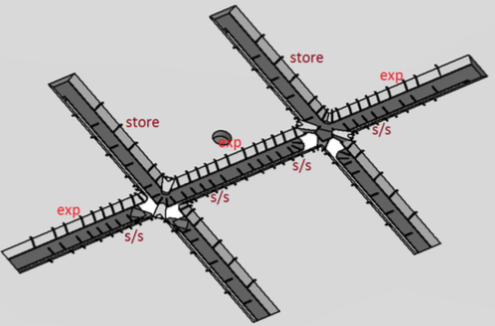
\includegraphics[width=.99\textwidth]{images/trap}
	\caption{Ion trap overview (should be improved, just filling space now)}
\end{figure}

\section{Kinds of resonators}
\label{sec:kinds_resonators}
The required frequency of 40 MHz limits our selection to the following types of resonators: helical \cite{Gulde2017, Johnson2016, VanRynbach2016, Kassa2016, Kassa2017} or, for higher frequencies, coaxial \cite{Karin2012}, RLC \cite{Gandolfi2010, Kumph2015, Greene2016}, and crystal oscillators. Multiple available solutions require us to do an analysis for a reasoned choice.
\subsection{Helical}
\begin{figure}[h]
	\centering
	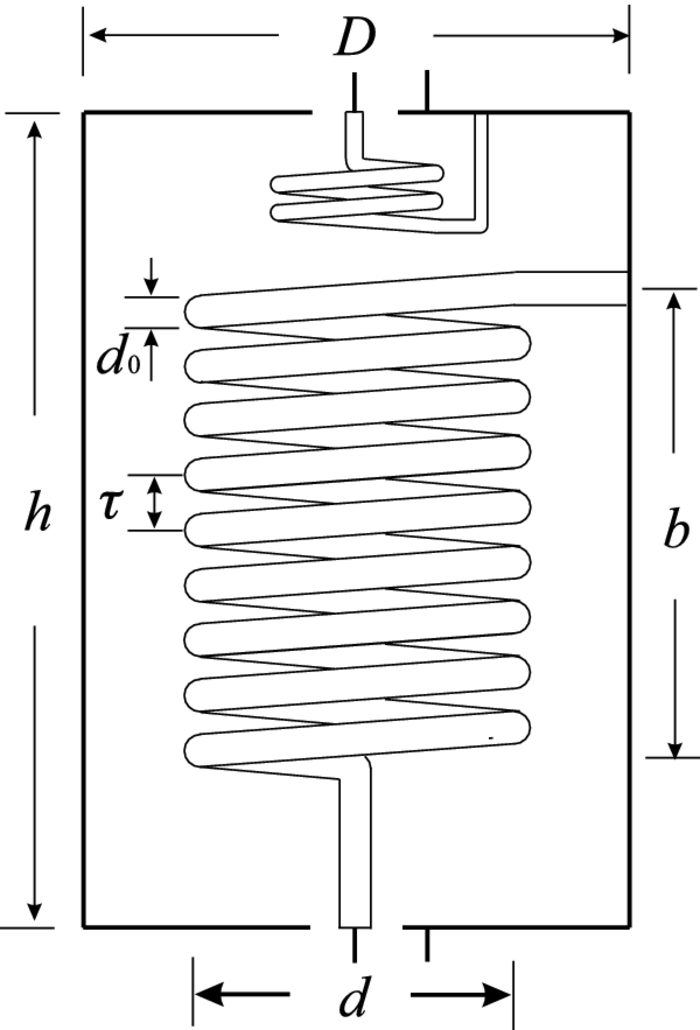
\includegraphics[width=.6\textwidth]{images/helical}
	\caption{Schematic diagram of a helical resonator indicating shield diameter $D$, shield height $h$, coil diameter $d$, coil height $b$, winding pitch $\tau$, and coil wire diameter $d_0$. \cite{Deng2014}}
	\label{fig:helical_example}
\end{figure}

Helical resonators are commonly selected to be coupled with ion traps due to their high quality factors and ability to operate on high frequencies. It is a perfect option for ion traps operated at room temperatures, since in absence of space constraints they are able to provide $Q$ values of a couple thousands. However in order to achieve those $Q$, the fabrication process needs to be quite precise to avoid reflections of traveling waves which negatively influence the overall gain.
\subsection{RLC}
\begin{figure}[h]
	\centering
	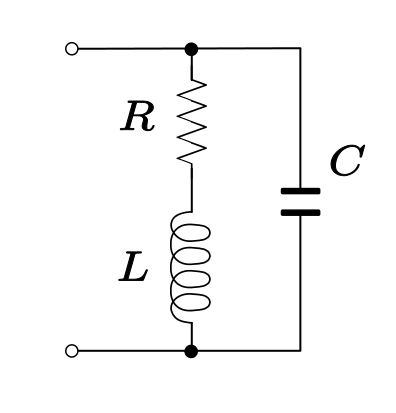
\includegraphics[width=.5\textwidth]{images/RLC}
	\caption{Example of a parallel RLC circuit}
\end{figure}

RLC amplifiers are a convenient choice for space-bounded environments, such as cryostats. Typical implementation pumps energy between two reactive components --- inductor and capacitor. Assembly of RLC circuit is easier than of helical resonator since the physical placement of lumped parts does not influence the resulting quality factor. But it also means that the quality of these components is a major factor for successful creation. Given that units' data sheets rarely provide values for cryogenic setup it takes a lot of trial and error to find the right ones \cite{Gandolfi2010}.
\subsection{Crystal}
Unlike helical and RLC resonators, the crystal oscillators do not store energy just in the electric field. This type or resonator utilizes piezoelectric effect to transform applied harmonic voltage into surface mechanical modes and vice versa.

Narrow excitation spectrum is provided by physical dimensions imposing hard constraints on vibrational oscillations and could have made such device an ideal filtering solution for ions traps. Unfortunately, there are some major downsides that seriously limit its applicability:
\begin{itemize}
	\item after fabrication resonant frequency can not be widely tuned
	\item limited stability of the crystal does not allow high voltages
\end{itemize}
\subsection{Choosing the right one}
In our setup, the combination of high voltage and frequency values with our constraints on available space makes helical resonator the optimal option. However, difficulties of assembly do not make it a perfect solution in terms of scalability --- for a production-grade setup RLC amplifier might be preferred.

[4K CHAMBER PIC HERE]
\chapter{Theory}

\section{Helical resonator models}
In order to create a helical resonator satisfying experimental conditions and limitations we inevitably come to a need for a theoretical model that would be able to predict essential characteristics of a resulting unit. The following sections aim to provide an overview and comparison of those.

\subsection{Macalpine}
A well-known approach \cite{Macalpine2000} for describing helical resonators was introduced in the same year 1959 as Richard Feynman's idea \cite{Feynman1960} to use quantum systems for computations. It grew from the possibility to reduce volume compared to TEM-mode coaxial-line resonators.

\subsection{Hensinger}
This model \cite{Siverns2012} takes one step further to designing an amplifier specifically for the needs of quantum computing. Authors propose to take a look at the joint resonator--ion trap system as a whole. It allows to calculate proper resonant frequency, accounting for resistive losses.


\section{Comparison}

Macalpine uses a generic model for coaxial / helical resonator, later improving it by using telegrapher's equations to estimate resonant frequency shift. Hensinger takes a less generic approach, taking some resonator-only parameters from Macalpine but investigating helical resonator + ion trap system
\chapter{Design}

Started
\chapter{Validation}

Two parameters defining the assembled resonator are the central frequency $\omega_0$ and the quality factor $Q$. In this chapter we measure their experimental values and compare to those defined in the table \ref{tbl:restrictions_siverns}.

\section{Measurements}

In order to determine $\omega_0$ and $Q$ we would take a look at the reflection spectrum of the system consisting of resonator + coaxial cable + capacitor. For every configuration the depth of the resonance was optimized by changing the distance and the angle between the antenna mount \ref{subsection:antenna_mount} and the top cap \ref{subsection:cap_top}, effectively adjusting the antenna to coil coupling. 

\begin{table}[h]
\centering
\begin{tabular}{| l | l | r | r |}
	\hline
	Parameter & Definition & Values & Units\\
	\hline \hline
	$C_{load}$ & External capacitive load & $10,15,22$ & pF\\
	\hline
	$L_{coax}$ & Length of the coaxial cable & $10, 20, 50$ & cm\\
	\hline
\end{tabular}
\label{tbl:experimental_parameters}
\caption{Additional experimental parameters}
\end{table}

At the time of writing there is no clear values for the capacitance of the trap and the length of the wires connecting it with the resonator. By using a set of parameters defined in the table \ref{tbl:experimental_parameters} we aim to measure $\omega_0$ and $Q$ in the region similar to the one used for the numerical calculations and broad enough to include the point $\{C_{load} = C_{trap}; L_{coax}\}$ of the final setup.

\begin{itemize}
	\item For $L_{coax}=50$ two coaxial cables were connected, introducing 2 additional SMA connectors to the contour
	\item Available SMA connectors were of the male type. Unfortunately it is also the type commonly used for the wires, so we had to use an additional female-female adapter (+1 for $L_{coax} = 50$)
\end{itemize}

\begin{figure}[h]
	\centering
	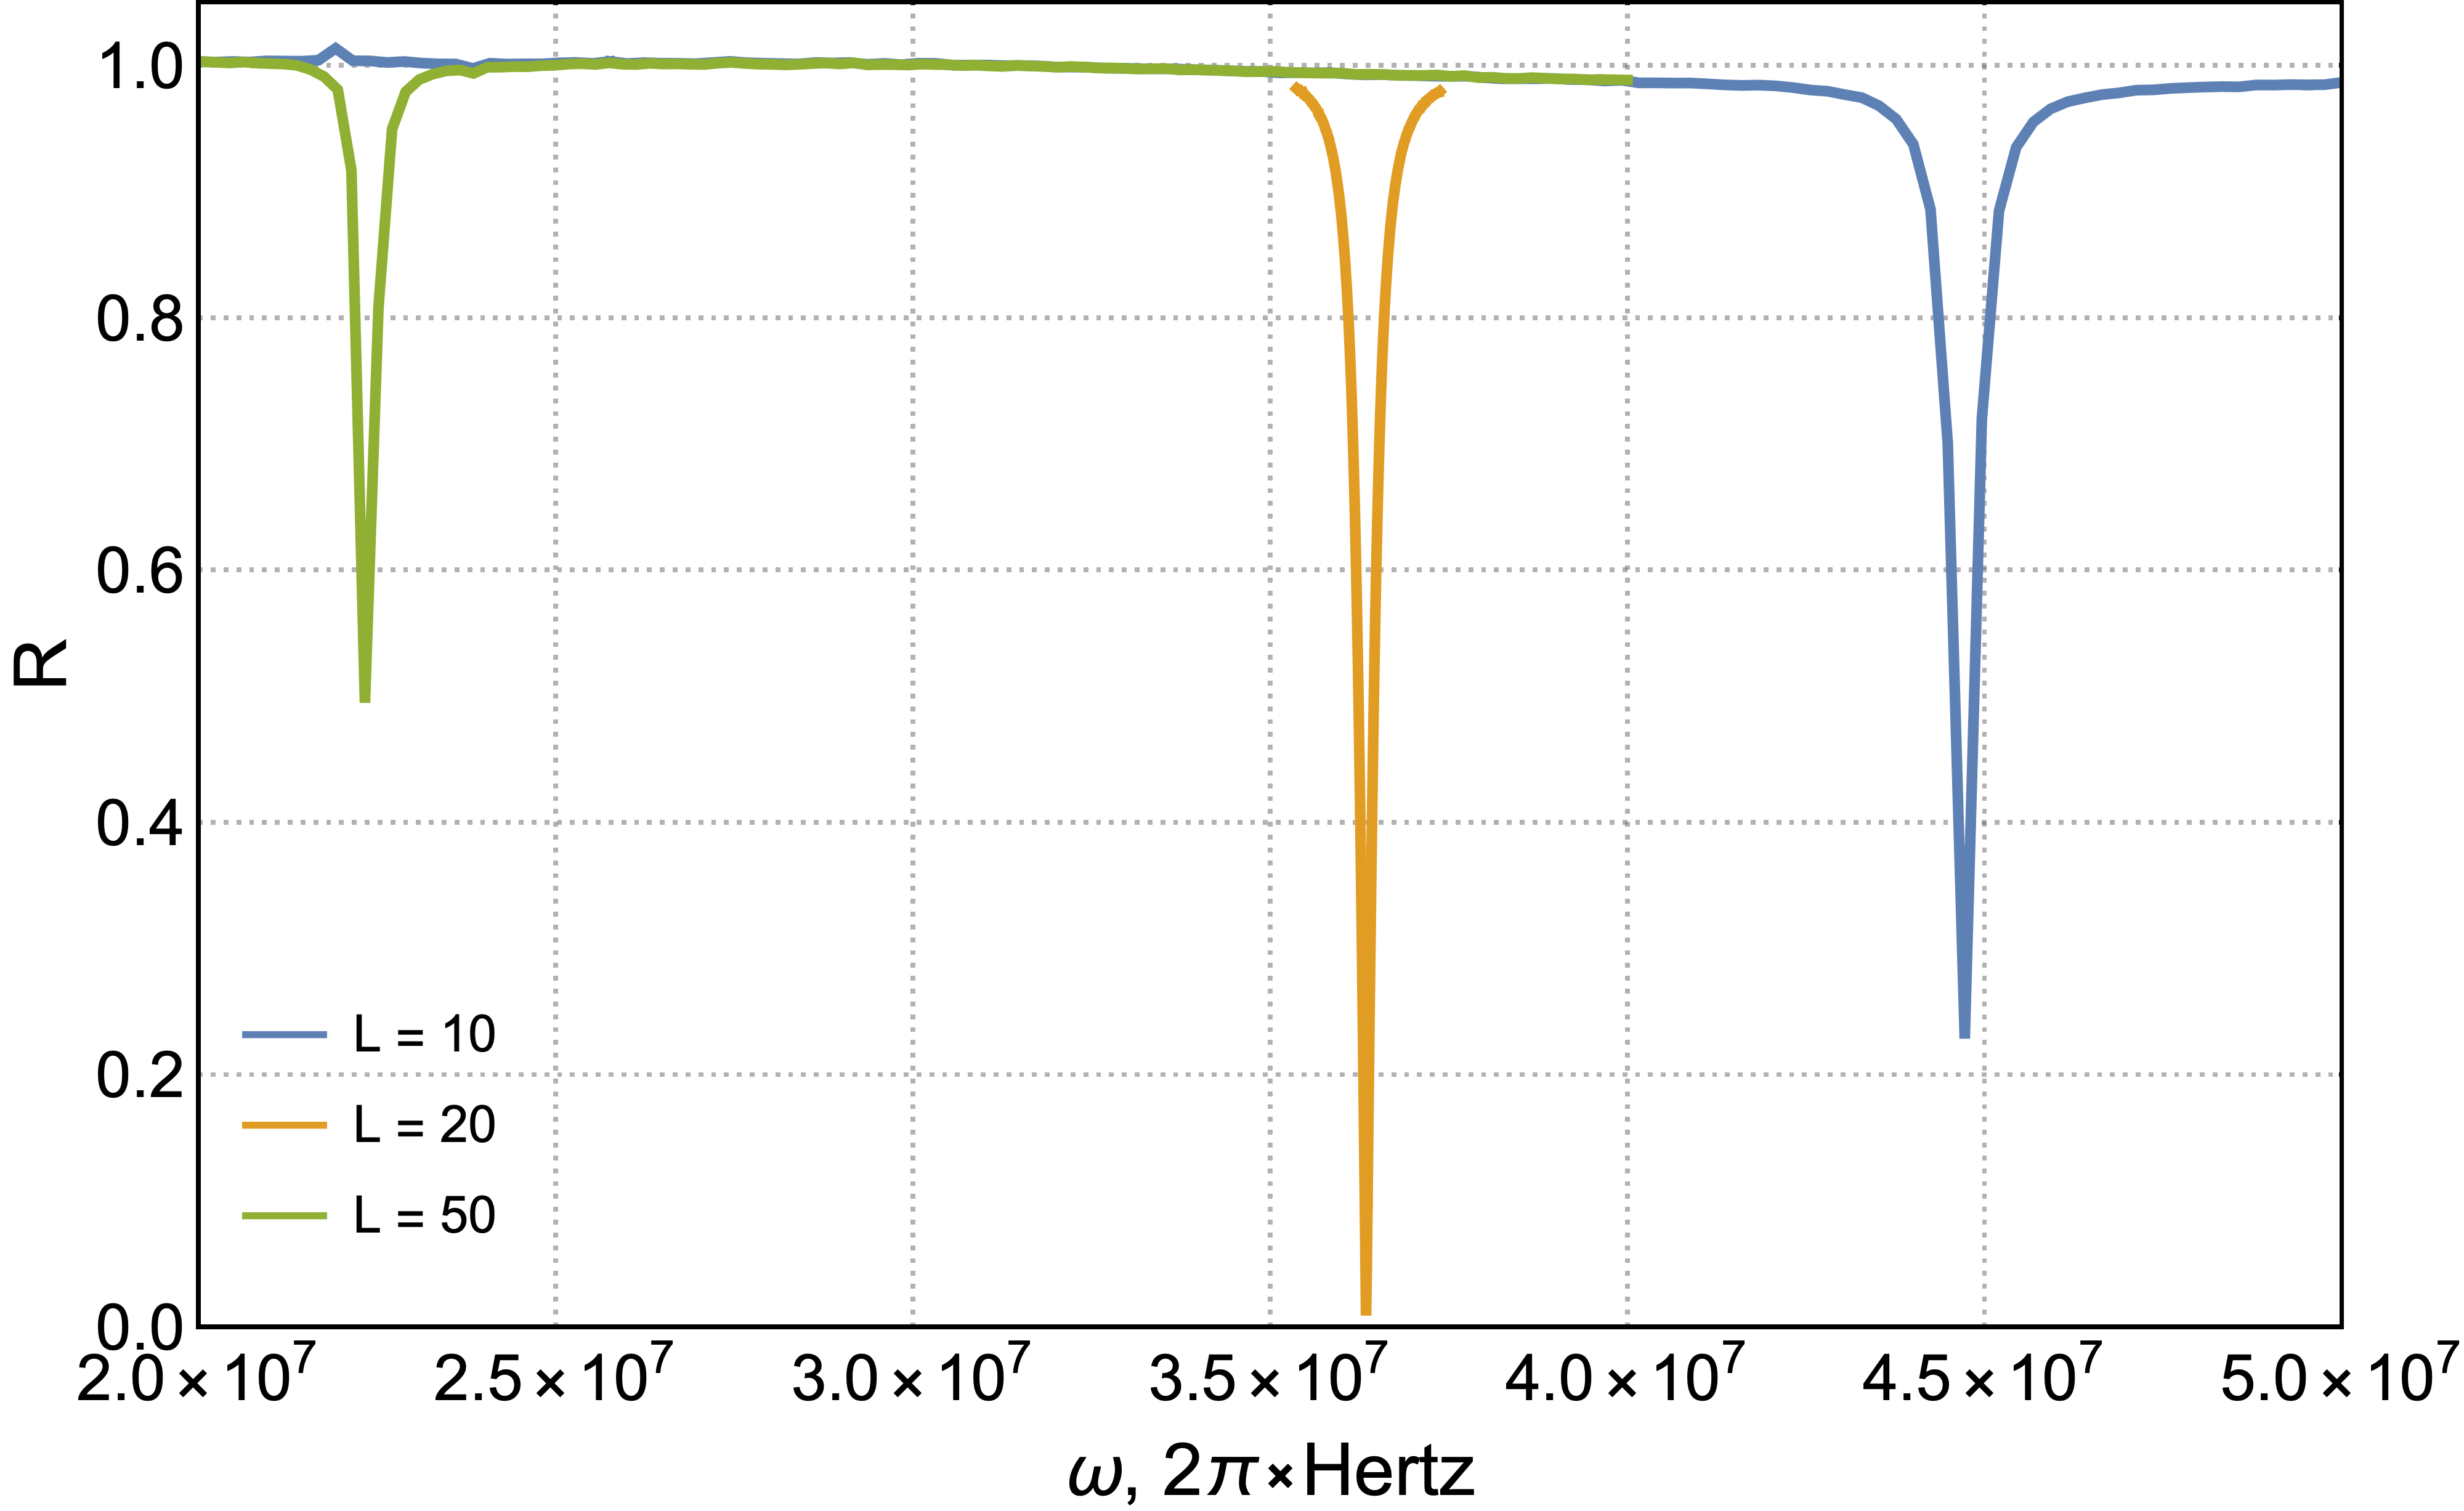
\includegraphics[width=\textwidth]{images/R_plot_C_10}
	\label{fig:R_C_10}
	\caption{Reflection spectrum for $C = 10$}
\end{figure}
\begin{figure}[h]
	\centering
	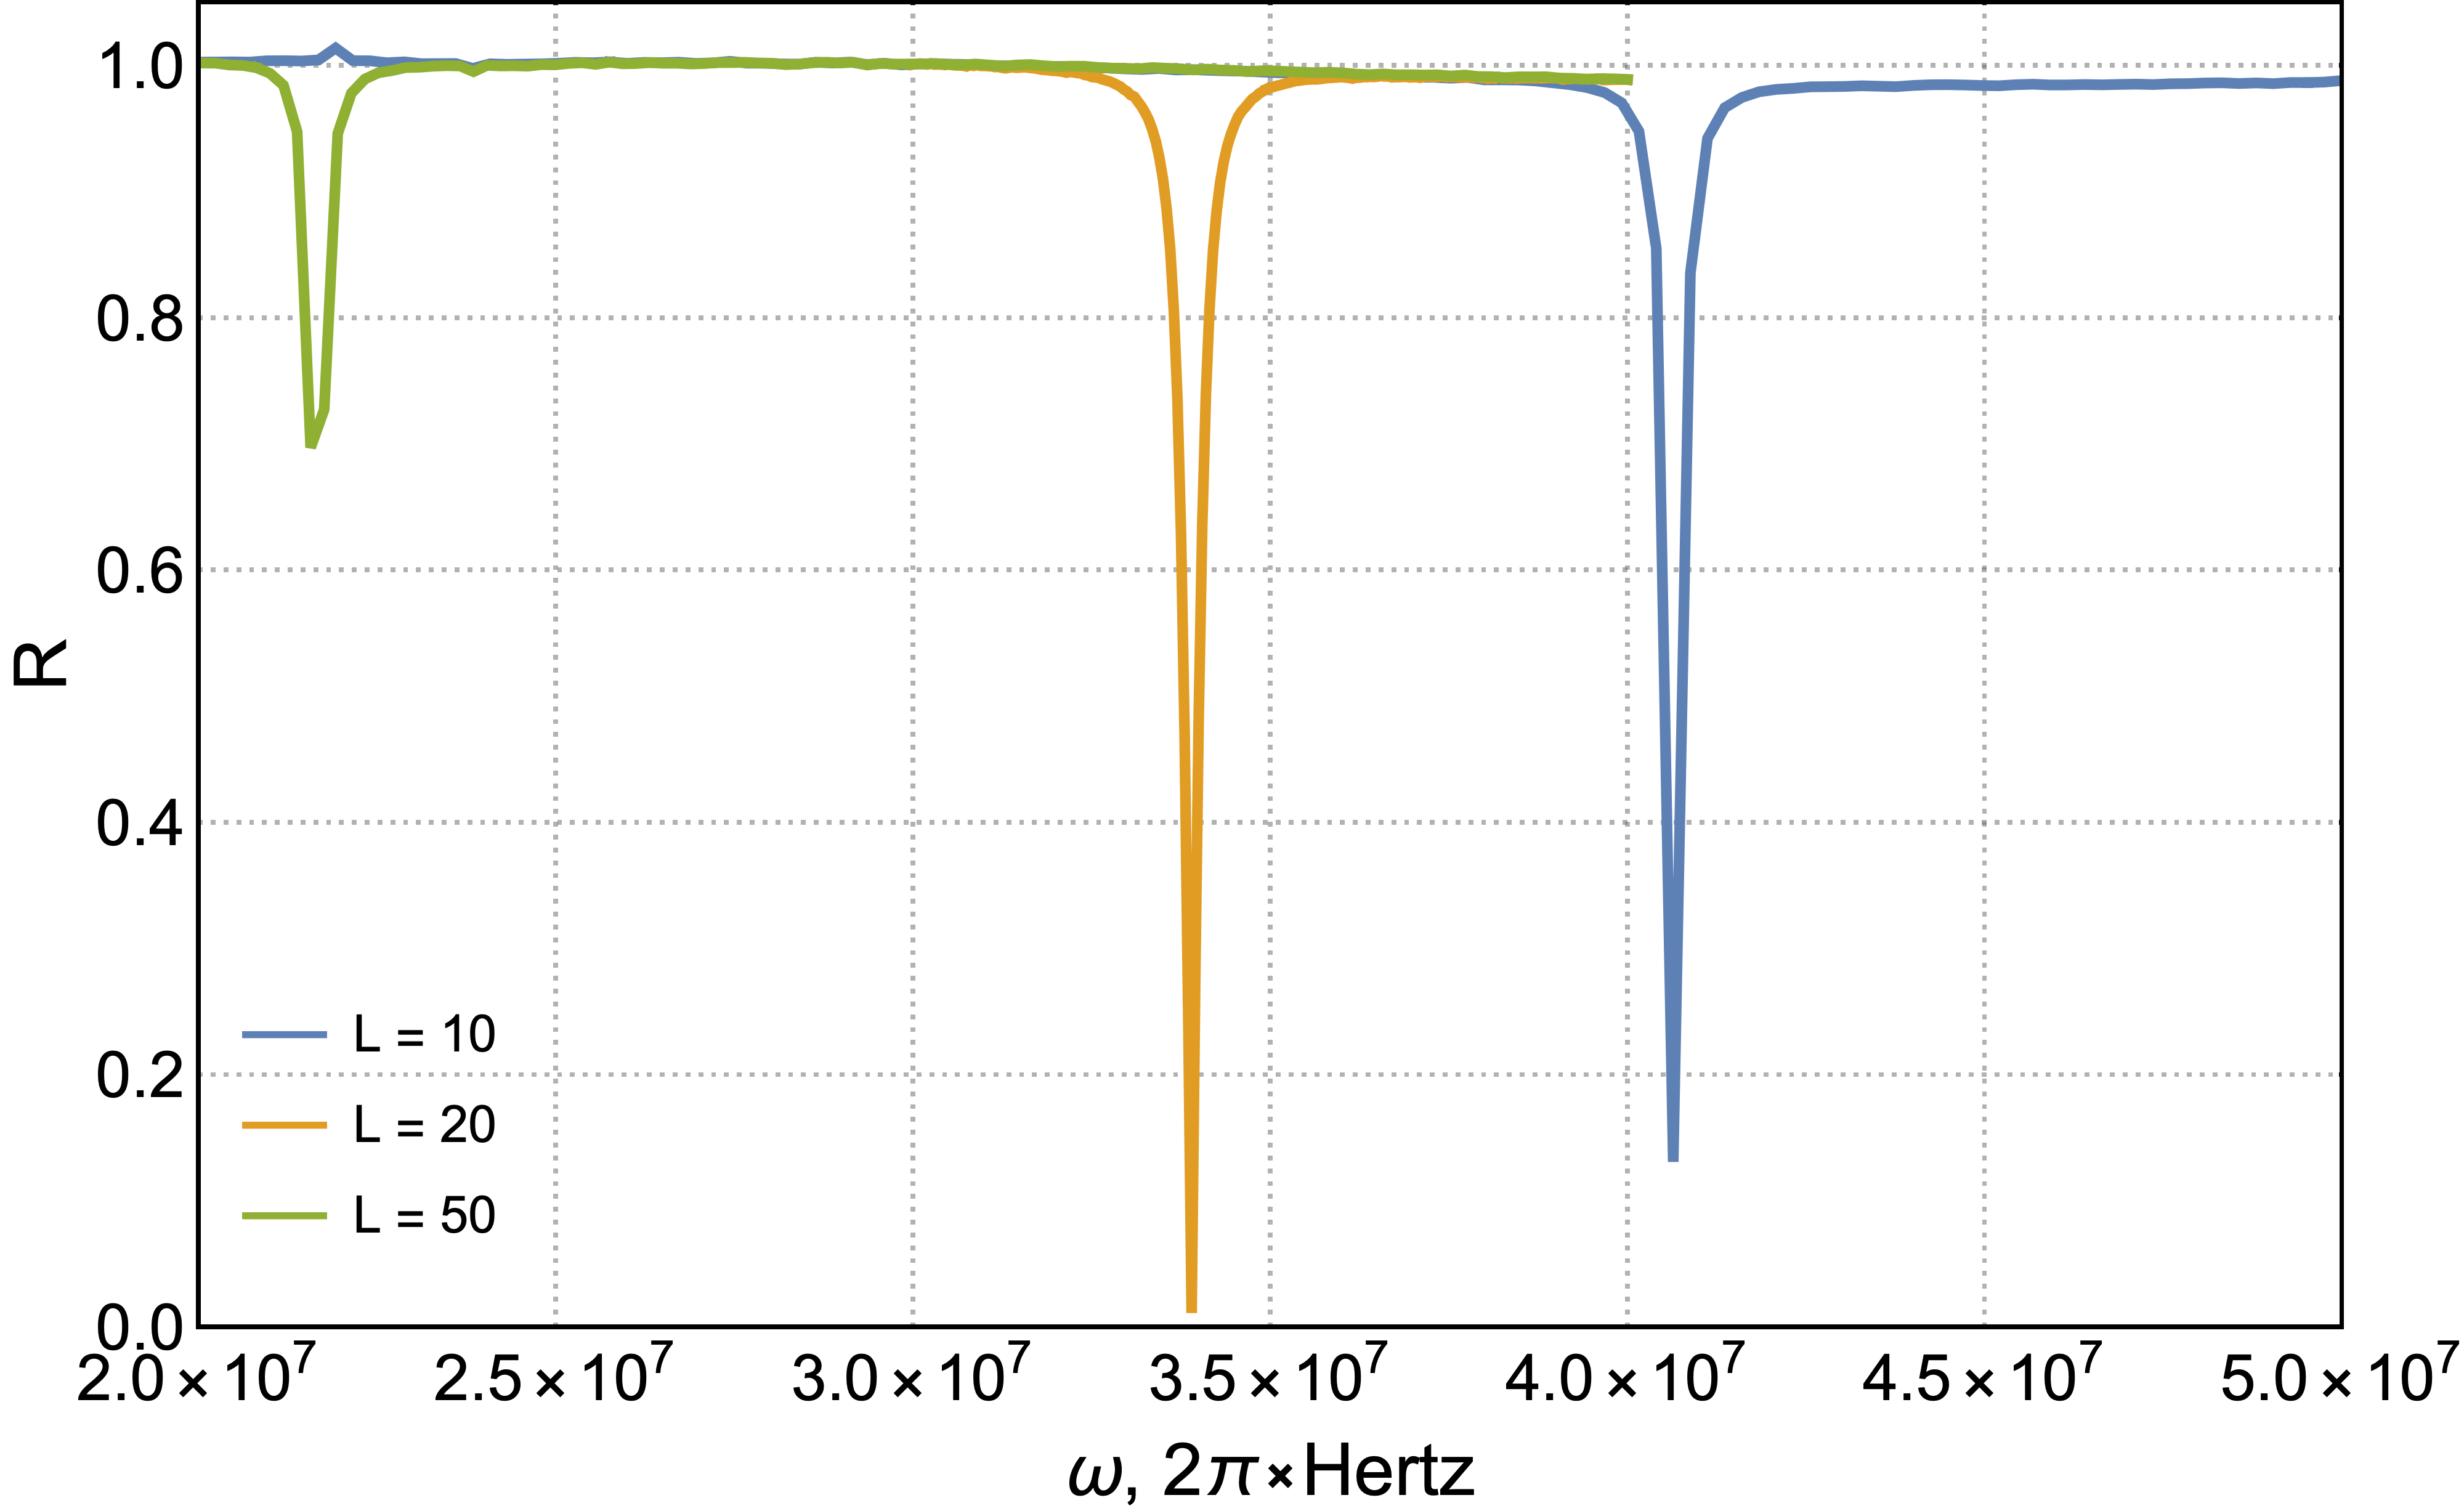
\includegraphics[width=\textwidth]{images/R_plot_C_15}
	\label{fig:R_C_10}
	\caption{Reflection spectrum for $C = 15$}
\end{figure}
\FloatBarrier
\begin{figure}[h]
	\centering
	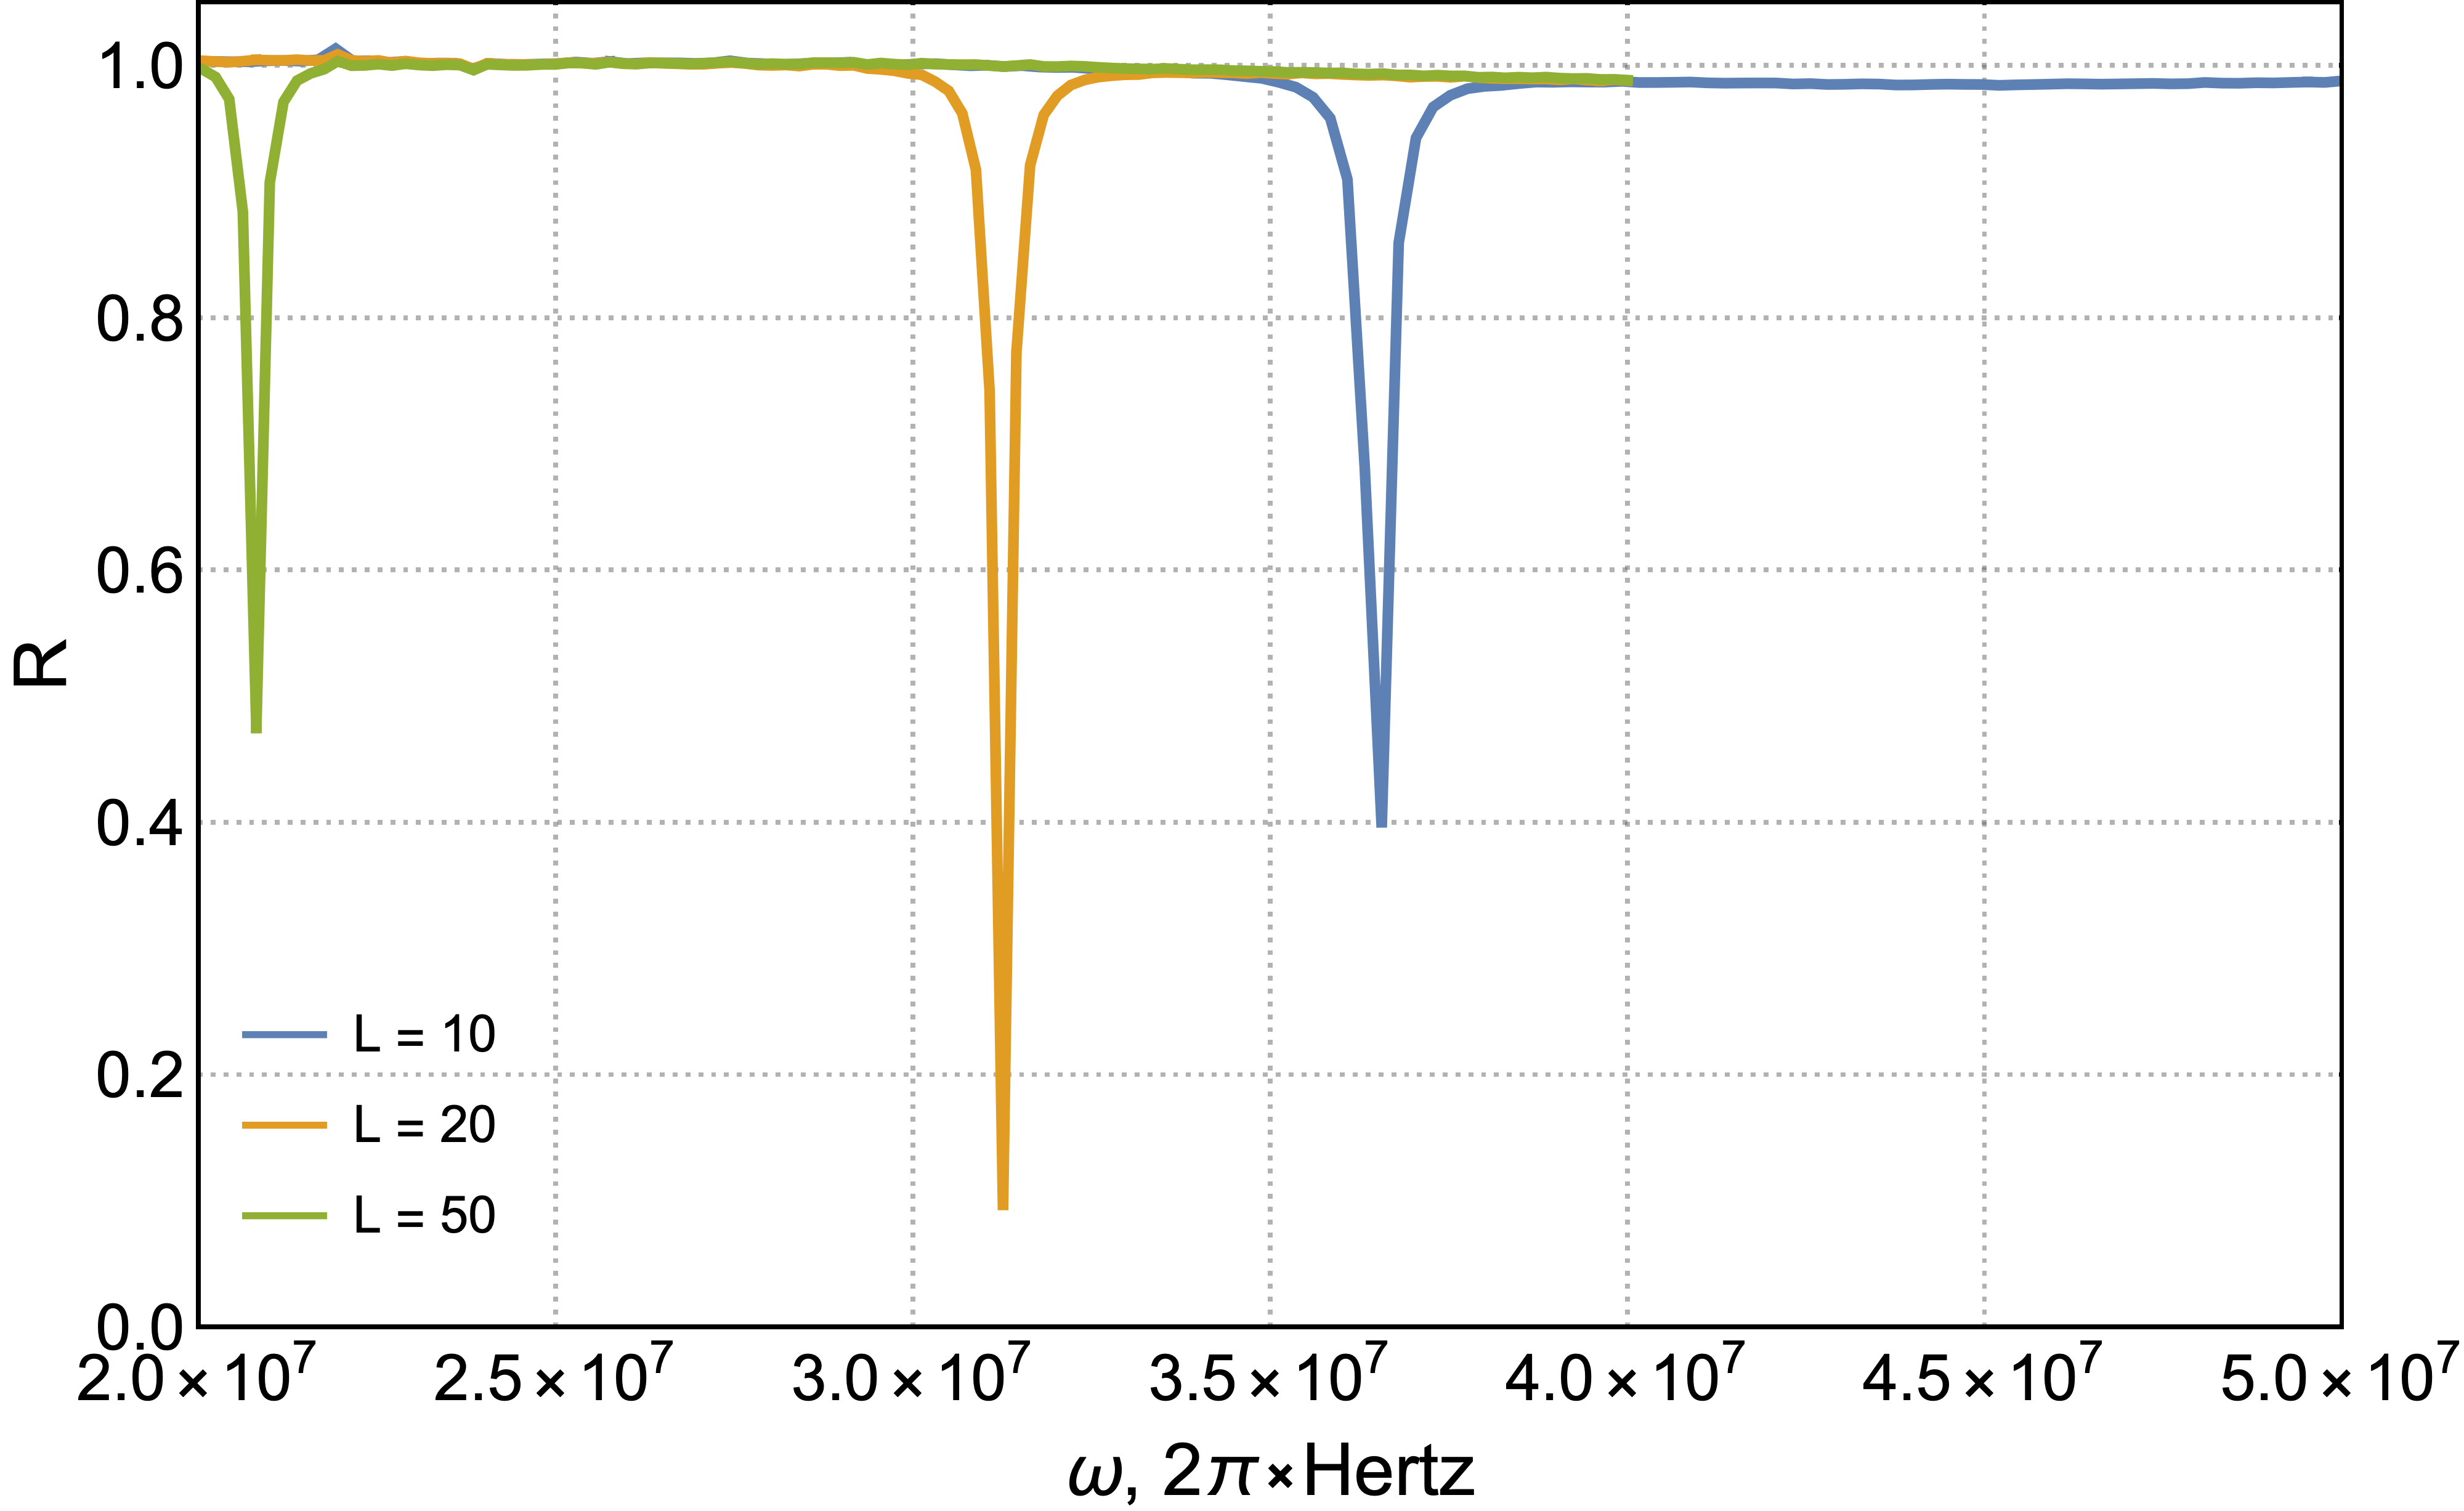
\includegraphics[width=\textwidth]{images/R_plot_C_22}
	\label{fig:R_C_10}
	\caption{Reflection spectrum for $C = 22$}
\end{figure}
\origsection{Analysis}
\FloatBarrier
Finding $\omega_0$ from experimental data is trivial, it is the central frequency of the peak. For the transmission spectrum $Q$ can be defined as
\begin{equation}
	Q = \frac{\omega_0}{\Delta \omega},
\end{equation}
where $\Delta \omega$ is the width of the peak at the $1/\sqrt{2}$ height. Since we are working with the reflection spectrum we need to adjust the height using the following expression
\begin{equation}
	R_{1/\sqrt{2}} = 1 - \frac{1 - R_{peak}}{\sqrt{2}}.
	\label{eq:reflection_height}
\end{equation}

Measured values of $\omega_0$ and $Q$ are presented in the table \ref{tbl:Q_w_results}. Visual comparison with the predicted values from the table \ref{tbl:restrictions_siverns} is shown in the chart \ref{fig:Q_w_deviation}. $C_{load} = 22$ pF is not equal to the simulated $C_{trap} = 20$ pF but was considered being close enough. The closer experimental data is to the point $\{0; 0\}$ the better it reflects the simulations. It can be seen that increased capacitance due to both $C_{load}$ and $L_{coax}$ tends to increase deviations from predictions.
\begin{table}[h]
\centering
\begin{tabular}{| r | r || r | r || r | r |}
	\hline
	$C_{load}$, pF & $L_{coax}$, cm & $\omega^{simul}_0$, $2\pi*$MHz & $\omega_0$, $2\pi*$MHz & $Q^{simul}$ & $Q$\\
	\hline \hline
	10 & 10 & 44.6 & 44.7 & 418 & 223.5\\
	\hline
	10 & 20 & \dittotikz & 36.3 & \dittotikz & 269.9\\
	\hline
	10 & 50 & \dittotikz & 22.3 & \dittotikz & 140.4\\
	\hline
	15 & 10 & 45.6 & 40.6 & 360 & 216.5\\
	\hline
	15 & 20 & \dittotikz & 33.9 & \dittotikz & 268.6\\
	\hline
	15 & 50 & \dittotikz & 21.6 & \dittotikz & 69.7\\
	\hline
	22 & 10 & 46.9 & 36.5 & 311 & 153.5\\
	\hline
	22 & 20 & \dittotikz & 31.2 & \dittotikz & 192.3\\
	\hline
	22 & 50 & \dittotikz & 20.8 & \dittotikz & 145.6\\
	\hline
\end{tabular}
\label{tbl:Q_w_results}
\caption{Measured $Q$ and $\omega_0$ for various configurations}
\end{table}

\begin{figure}[h]
	\centering
	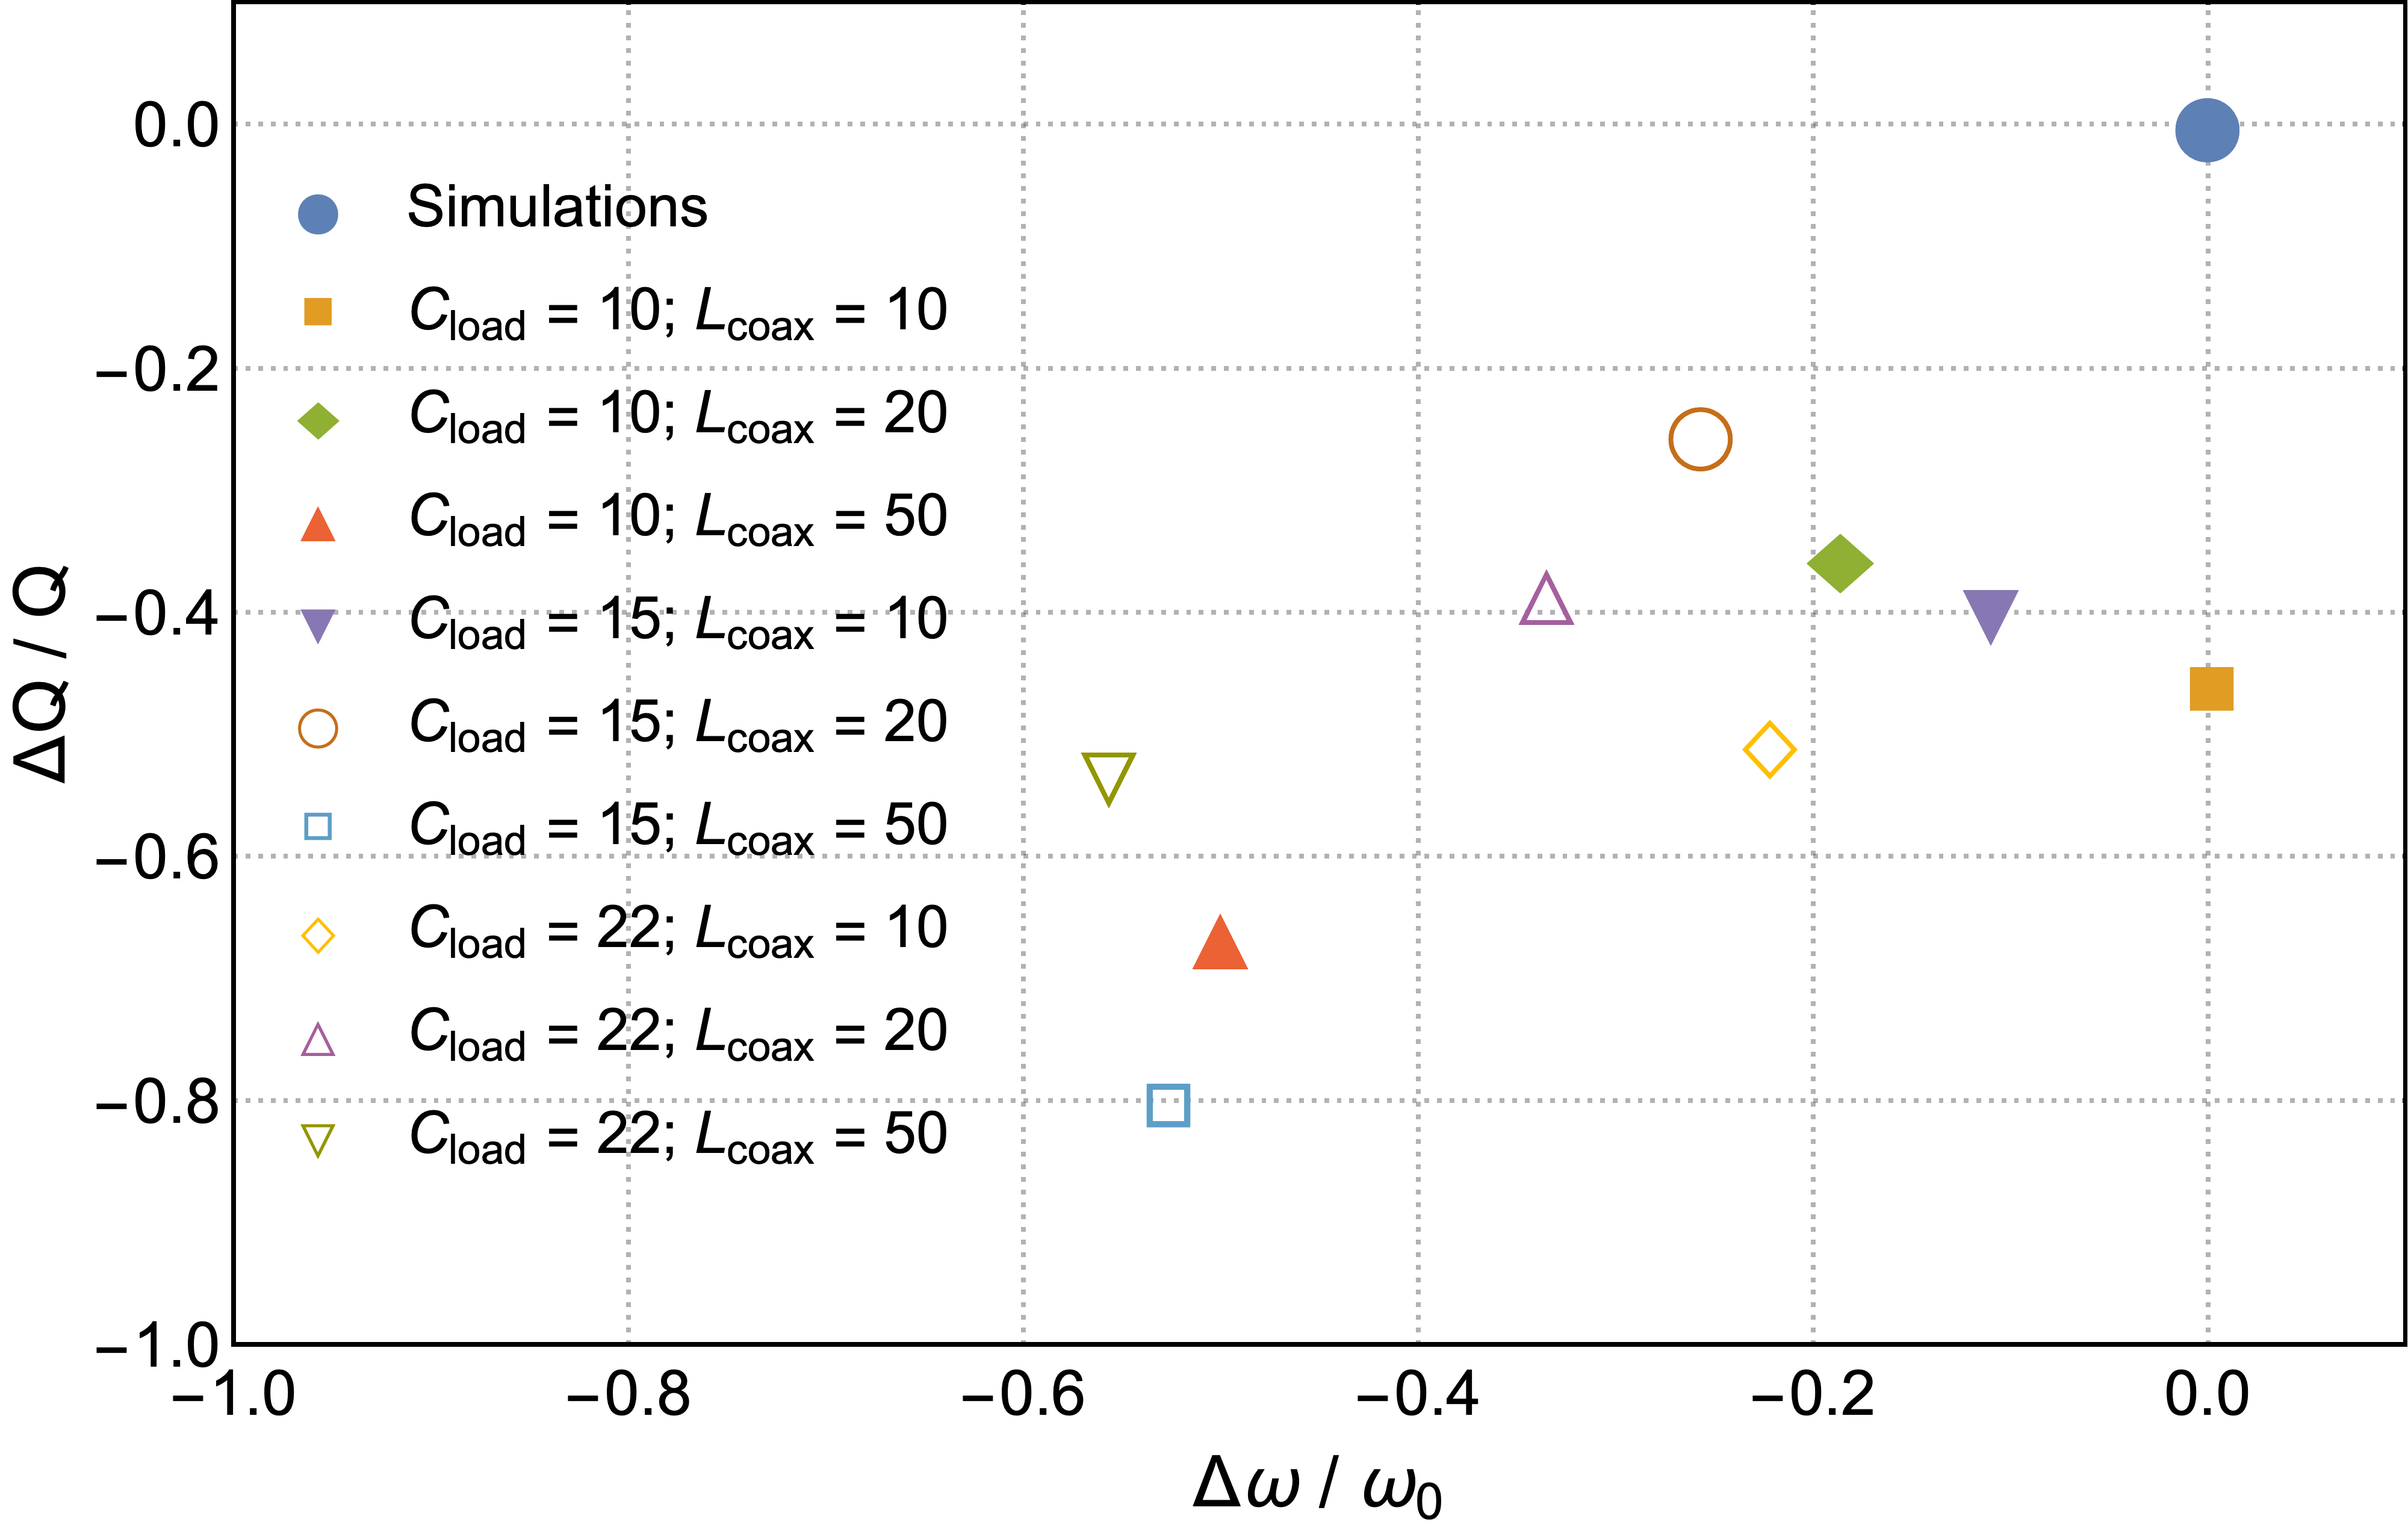
\includegraphics[width=\textwidth]{images/Q_w_plot}
	\label{fig:Q_w_deviation}
	\caption{Relative deviations of $Q$ and $\omega_0$}
\end{figure}

\section{Ideal drive}
This section includes simulations of the ideal drive for a 300 and 320 V drive by Chiara Decaroli.

\begin{figure}[h]
	\centering
	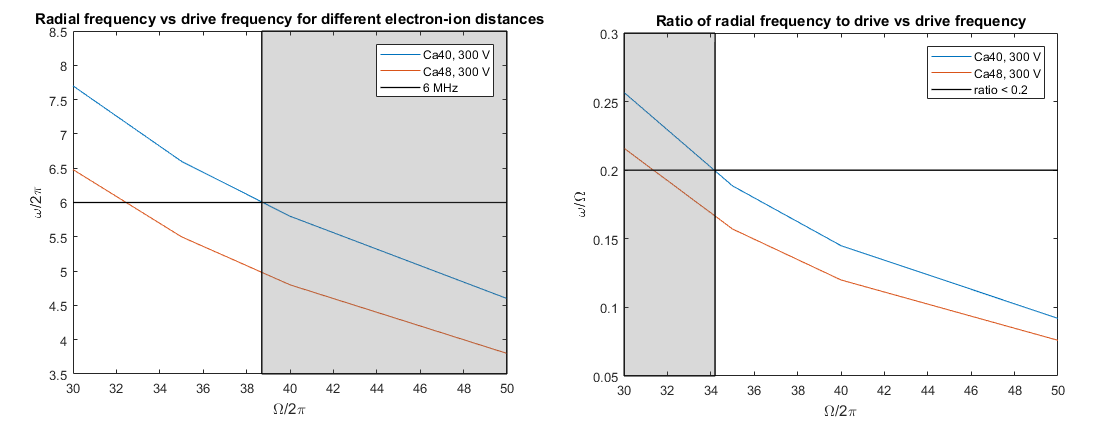
\includegraphics[width=\textwidth]{images/300Vcalcium}
	\label{fig:ideal_drive_300}
	\label{Simulation of the ideal drive for 300V}
\end{figure}
\begin{figure}[h]
	\centering
	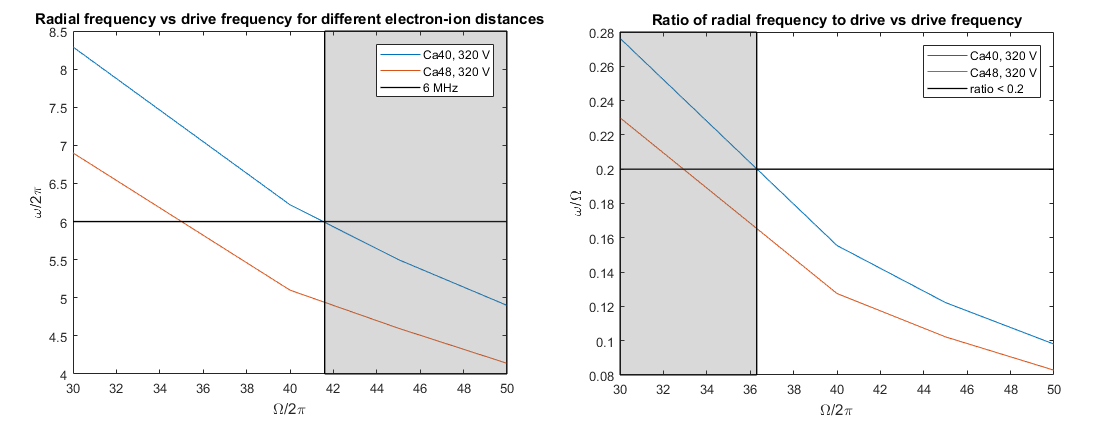
\includegraphics[width=\textwidth]{images/320Vcalcium}
	\label{fig:ideal_drive_320}
	\label{Simulation of the ideal drive for 320V}
\end{figure}
\chapter{Conclusion}

As a result of this project we were able to implement a delicate helical resonator with reasonable $Q$ and $\omega_0$ values. There is definitely room for improvement:

\begin{itemize}
	\item Angular tuning didn't prove to work, which is also good since it shows that structure is fairly symmetrical to rotations.
	\item Distance tuning almost didn't work, for an optimal tuning the distance between the antenna mount was kept close to 0. Possible solution would be either to add another turn to the antenna itself or extend the length of the antenna mount to gain more flexibility.
	\item Helical resonator has spent a fair share of time being in contact with air. Cleaning the internal surface of the shield with sanding or acid should remove oxidized layer of copper and improve conductivity.
	\item SMA adapters are good for testing and probing the device, but add additional capacitance ––– for a usage with a real trap it would be recommended to solder the wires directly.
	\item Coaxial cables also add capacitance, better results might be achieved with using regular wires.
	\item Theoretical calculations used conductivity at cryogenic temperatures, moving the helical resonator into the cryostat should provide results closer to those expected from the model.
\end{itemize}
%\chapter{External circuits \& additional features}

\appendix

\chapter{Mathematica code for Macalpine's model}
\label{chapter:macalpine_code}
This is a relevant part of the script supporting calculations in \cite{Leupold2015}.
\begin{mmaCell}[moredefined={c, AMU, h, kB, grav, a0, me, ee, eV, Eh, m, mm, cm, nm, km, in, ft, mi, mK, nK, pK, T, mT, G, mG, sec, s, ms, ns, A, mA, nA, W, mW, nW, Hz, kHz, MHz, GHz, nF, pF, nH, pH}]{Input}
(* Physical Constants and Units *)
\mmaDef{\(\mu\)0} = 4*\mmaDef{\(\pi\)}*\mmaSup{10}{-7};
\mmaDef{\(\epsilon\)0} = 8.854187817*\mmaSup{10}{-12};
c = 299792458;
AMU = 1.6605402*\mmaSup{10}{-27};
h = 6.6260755*\mmaSup{10}{-34};
\mmaDef{\(\hbar\)} = \mmaFrac{h}{2\mmaDef{\(\pi\)}};
\mmaDef{\(\mu\)B} = 9.2740154*\mmaSup{10}{-24};
kB = 1.380658*\mmaSup{10}{-23};
grav = 9.8;
a0 = 0.5291772108*\mmaSup{10}{-10};
me = 9.1093826*\mmaSup{10}{-31};
ee = 1.60217733*\mmaSup{10}{-19}; eV = ee;
Eh = \mmaFrac{\mmaSup{\mmaDef{\(\hbar\)}}{2}}{me \mmaSup{a0}{2}};
m=1; \mmaDef{\(\mu\)m}=\mmaSup{10}{-6}m; mm=\mmaSup{10}{-3}m; cm=\mmaSup{10}{-2}m; nm=\mmaSup{10}{-9}m; km=\mmaSup{10}{3}m;
in=2.54cm; ft=12in; mi=5280*ft;
K=1; mK=\mmaSup{10}{-3}K; \mmaDef{\(\mu\)K}=\mmaSup{10}{-6}; nK=\mmaSup{10}{-9}K; pK=\mmaSup{10}{-12};
T=1; mT=\mmaSup{10}{-3}K; G=\mmaSup{10}{-4}; mG=\mmaSup{10}{-3}G; \mmaDef{\(\mu\)G}=\mmaSup{10}{-6};
sec=1; s=1; ms=\mmaSup{10.0}{-3}s; \mmaDef{\(\mu\)s}=\mmaSup{10}{-6}s; ns=\mmaSup{10}{-9}s;
\mmaDef{\(\Omega\)}=1; \mmaDef{m\(\Omega\)}=\mmaSup{10}{-3}; \mmaDef{k\(\Omega\)}=\mmaSup{10}{3}; \mmaDef{M\(\Omega\)}=\mmaSup{10}{6};
A=1; mA=\mmaSup{10}{-3}A; \mmaDef{\(\mu\)A}=\mmaSup{10}{-6}; nA=\mmaSup{10}{-9};
W=1; mW=\mmaSup{10}{-3}; \mmaDef{\(\mu\)W}=\mmaSup{10}{-6}; nW=\mmaSup{10}{-9};
Hz=1; kHz=\mmaSup{10}{3}; MHz=\mmaSup{10}{6}; GHz=\mmaSup{10}{9};
nF=\mmaSup{10}{-9}; pF=\mmaSup{10}{-12};
nH=\mmaSup{10}{-9}; pH=\mmaSup{10}{-12};
\end{mmaCell}

\begin{mmaCell}[moredefined={Ds, d, b, Nt, d0, Leff, Ceff, Z0, v, Q, omega},morepattern={Bs_, Bs, f0_, f0, Cl_, Cl},morelocal={w}]{Input}
(* Calculations for Cu resonator *)
Ds[Bs_]:= 0.75Bs; (*diameter of shield*)
d[Bs_]:= 0.55Ds[Bs]; (*diameter of helix*)
b[Bs_]:= 1.5d[Bs]; (*length of helix*)

Nt[Bs_,f0_]:= \mmaFrac{48.26*\mmaSup{10}{6}}{f0 Ds[Bs]}; (*number of turns*)

d0[Bs_,f0_]:= 0.5\mmaFrac{b[Bs]}{Nt[Bs, f0]}; (*diameter of wire*)

\mmaDef{\(\tau\)}[Bs_,f0_]:= \mmaFrac{b[Bs]}{Nt[Bs, f0]}; (*pitch*)

(*effective inductance*)
Leff[Bs_,f0_]:= 9.84*\mmaSup{10}{-7}*\mmaSup{(\mmaFrac{Nt[Bs, f0] d[Bs]}{b[Bs]})}{2}*(1-\mmaSup{(\mmaFrac{d[Bs]}{Ds[Bs]})}{2});
Ceff[Bs_]:= \mmaFrac{2.95*\mmaSup{10}{-11}}{Log[10,\mmaFrac{Ds[Bs]}{d[Bs]}]}; (*effective capacitance*)
  

Z0[Bs_,f0_]:= \mmaSqrt{\mmaFrac{Leff[Bs,f0]}{Ceff[Bs]}}; (*characteristic impedance*)

v[Bs_,f0_]:= \mmaFrac{1}{\mmaSqrt{Leff[Bs,f0] Ceff[Bs]}}; (*velocity*)
  
\mmaDef{\(\lambda\)}[Bs_,f0_]:= \mmaFrac{v[Bs,f0]}{f0}; (*wavelength*)

Q[Bs_,f0_]:= 1.97 Ds[Bs] \mmaSqrt{f0};

omega[Bs_,f0_,Cl_]:= Module[\{w\},
  w = \mmaUnd{\(\nu\)}/.FindRoot[\mmaFrac{1}{2\mmaDef{\(\pi\)}*Z0[Bs,f0]*Cl*\mmaFnc{\(\nu\)}}==Tan[\mmaFrac{2\mmaDef{\(\pi\)}\mmaFnc{\(\nu\)} b[Bs] }{v[Bs,f0]}],\{\mmaFnc{\(\nu\)},f0\}][[1]];
  Return@w;
]
\end{mmaCell}

\begin{mmaCell}[moredefined={mm, MHz, pF, Ds, d, b, Nt, d0, Z0, Leff, nH, Ceff, v, m, s, Q, omega}]{Input}
Bs = 60mm; (*length of shield*)
(* This frequency needs to be varied 
until loaded frequency is close to target frequency*)
f0 = 97.023MHz; (*center frequency*)
Cl = 10pF; (*trap capacitance*)
  
Print["Bs = ",Bs/mm," mm (length of shield)"]
Print["Ds = ",Ds[Bs]/mm," mm (diameter of shield)"]
Print["d = ",d[Bs]/mm," mm (diameter of helix)"]
Print["b = ",b[Bs]/mm," mm (length of helix)"]
Print["Nt = ",Nt[Bs,f0]," (number of turns)"]
Print["d0 = ",d0[Bs,f0]/mm," mm (diameter of wire)"]
Print["\(\tau\) = ",\mmaDef{\(\tau\)}[Bs,f0]/mm," mm (pitch of helix)"]
Print["Z0 = ",Z0[Bs,f0]/\mmaDef{\(\omega\)}," \(\omega\) (characteristic impedance)"]
Print["Leff = ",Leff[Bs,f0]/(nH/mm)," nH/mm (effective inductance)"]
Print["Ceff = ",Ceff[Bs]/(pF/mm)," pF/mm (effective capacitance)"]
Print["v = ",v[Bs,f0]/(m/s)," m/s (velocity)"]
Print["\(\lambda\) = ",\mmaDef{\(\lambda\)}[Bs,f0]/mm," mm (wavelength)"]
Print["f0 = ",f0/MHz," MHz (unloaded frequency)"]
Print["Q = ",Q[Bs,f0]," (quality factor)"]
Print["\(\nu\)0 = ",omega[Bs,f0,Cl]/MHz," MHz (loaded frequency)"]
  
Clear[Bs,f0,Cl];
\end{mmaCell}

\begin{mmaCell}{Print}
Bs = 60 mm (length of shield)
\end{mmaCell}

\begin{mmaCell}{Print}
Ds = 45. mm (diameter of shield)
\end{mmaCell}

\begin{mmaCell}{Print}
d = 24.75 mm (diameter of helix)
\end{mmaCell}

\begin{mmaCell}{Print}
b = 37.125 mm (length of helix)
\end{mmaCell}

\begin{mmaCell}{Print}
Nt = 11.0535 (number of turns)
\end{mmaCell}

\begin{mmaCell}{Print}
d0 = 1.67933 mm (diameter of wire)
\end{mmaCell}

\begin{mmaCell}{Print}
\(\tau\) = 3.35866 mm (pitch of helix)
\end{mmaCell}

\begin{mmaCell}{Print}
Z0 = 572.731 \(\Omega\) (characteristic impedance)
\end{mmaCell}

\begin{mmaCell}{Print}
Leff = 37.2698 nH/mm (effective inductance)
\end{mmaCell}

\begin{mmaCell}{Print}
Ceff = 0.11362 pF/mm (effective capacitance)
\end{mmaCell}

\begin{mmaCell}{Print}
v = 1.53672*10^7 m/s (velocity)
\end{mmaCell}

\begin{mmaCell}{Print}
\(\lambda\) = 158.387 mm (wavelength)
\end{mmaCell}

\begin{mmaCell}{Print}
f0 = 97.023 MHz (unloaded frequency)
\end{mmaCell}

\begin{mmaCell}{Print}
Q = 873.205 (quality factor)
\end{mmaCell}

\begin{mmaCell}{Print}
\(\nu\)0 = 40. MHz (loaded frequency)
\end{mmaCell}
\chapter{Mathematica code for Siverns' model}
\label{chapter:siverns_code}
Following calculations are heavily based on a script generously provided by James David Siverns. All variables and references correspond to \cite{Siverns2012}.
\begin{mmaCell}[addtoindex=-3,moredefined={MHz, pF, mm, m, H}]{Input}
(* Units and constants *)
MHz = \mmaSup{10}{6};
pF = \mmaSup{10}{-12};
\(\Omega\) = 1;
mm = \mmaSup{10}{-3};
m = 1;
H = 1;
\(\mu\)0 = 4\(\pi\)*\mmaSup{10}{-7};
\end{mmaCell}

\begin{mmaCell}[moredefined={Cw, pF, Rt},morepattern={Ct_, Ct}]{Input}
(* Trap and wire values *)
Cw = 0.00001 pF; (* Wire to trap capacitance *)
Rt = 0.1 \(\Omega\); (* Trap resistance *)
C\(\Sigma\)[Ct_]:= Cw + Ct; (* Sum of above *)
\end{mmaCell}

\begin{mmaCell}[moredefined={calculateQ, pF, mm, m, H, Cw, MHz, Rt},morepattern={dMillimeters_, \#, dMillimeters, Ct_, Ct},morelocal={d0,
d, De, eN, b, Cc, KLc, KCs, Cs, LC, lc, r, Ns, ls, a, Rs, Rc, Rj, XLc, XCc, Xct, Xcw, XCs, Zcoil, ZE, Ztot, RealZ, Q, maxSize, log, Capacitance}]{Input}
calculateQ[dMillimeters_, \mmaPat{\(\gamma\)_}]:=Module[\{
  (* Arguments naming as in Siverns paper *)
  d0,\mmaLoc{\(\tau\)},d,De,\mmaLoc{\(\alpha\)},\mmaLoc{\(\rho\)},eN,b,Cc,KLc,KCs,Cs,LC,\mmaLoc{\(\omega\)0},\mmaLoc{\(\delta\)},lc,r,Ns,ls,a,
  Rs,Rc,Rj,XLc,XCc,Xct,Xcw,XCs,Zcoil,ZE,Ztot,RealZ,Q,
  maxSize, log, \mmaLoc{\(\omega\)Res}, Capacitance
\},
  Capacitance = 20pF;
  (* Switch log function for plotting *)
  log = Print;
  log = (#)&;
  
  (* Resonator parameters *)
  (* Coil wire diameter, we take it from Macalpine *)
  d0 = 1.95mm;
  \mmaLoc{\(\tau\)} = 2*d0; (* Winding pitch *)
  d = dMillimeters*mm; (* Diameter of coil *)
  De = d/\mmaPat{\(\gamma\)}; (* Diameter of a shield *)
  \mmaLoc{\(\alpha\)} = d/De;
  (* Resistivity of resonator material *)
  \mmaLoc{\(\rho\)} = 1.7*\mmaSup{10}{-8}*\mmaDef{\(\Omega\)}*m;  
  (* Given by the 4K chamber design *)
  maxSize = 36mm;
  b = 56mm - De/2;
  (* Handling case of a too large resonator *)
  If[d>maxSize || De>maxSize || b\(\pmb{\leq}\)0, Return@0];
  
  log["b = ", b/mm, "mm"];
  log["d = ", d/mm, "mm"];
  log["D = ", De/mm, "mm"];
  
  eN = b/\mmaLoc{\(\tau\)};(* Number of turns in the coil *)
  log["N = ", eN];
  (* Coil self capacitance - equation 25 *)
  
  Cc = ((11.26\mmaFrac{b}{d})+8+(\mmaFrac{27}{Sqrt[\mmaFrac{b}{d}]}))d pF;
  
  
  KLc = 39.37 \mmaFrac{0.025 \mmaSup{(d)}{2} (1-\mmaSup{\mmaLoc{\(\alpha\)}}{2})}{\mmaSup{(\mmaLoc{\(\tau\)})}{2}}\mmaSup{10}{-6}\mmaFrac{H}{m};
  
  KCs = 39.37 \mmaFrac{0.75}{Log[10,\mmaFrac{1}{\mmaLoc{\(\alpha\)}}]} \mmaFrac{pF}{m};
  
  (* Shield-coil capacitance - equation 26 *)
  Cs = b KCs;
  (* Inductance of coil inside a shield - equation 27 *)
  LC = b KLc;
  (* Resonant frequency - equation 21 *)
  \mmaLoc{\(\omega\)Res}[Ct_]:= \mmaFrac{1}{Sqrt[(Cs+Ct+Cw+Cc)LC]};
  
  log["\(\omega\) = ", \mmaLoc{\(\omega\)Res}[Capacitance]/(2\mmaDef{\(\pi\)} MHz), "MHz"];
  
  \mmaLoc{\(\omega\)0}[Ct_]:= 2\mmaDef{\(\pi\)}*40 MHz; (* This is a target frequency *)
  (* Allowing 15% accuracy for the frequency *)
  If[
  	\mmaFrac{Abs[\mmaLoc{\(\omega\)0}[Capacitance] - \mmaLoc{\(\omega\)Res}[Capacitance]]}{\mmaLoc{\(\omega\)0}[Capacitance]} > 0.15, 
  	Return@0
  ];
  
  \mmaLoc{\(\delta\)}[Ct_]:= Sqrt[\mmaFrac{2 \mmaLoc{\(\rho\)}}{(\mmaLoc{\(\omega\)0}[Ct] \mmaDef{\(\mu\)0} )}]; (* Skin depth *)
  
  (* Unwound length of the coil *)
  lc = 2\mmaDef{\(\pi\)} Sqrt[\mmaSup{(\mmaFrac{d}{2})}{2}+\mmaSup{(\mmaFrac{\mmaLoc{\(\tau\)}}{2\mmaDef{\(\pi\)}})}{2}]\mmaFrac{b}{\mmaLoc{\(\tau\)}};
  r = \mmaFrac{d}{2}(\mmaFrac{1}{\mmaLoc{\(\alpha\)}}-1);
  
  (* Number of "turns" in the currents path in the shield 
  - equation 31 *)
  
  Ns = \mmaFrac{b lc}{4\mmaDef{\(\pi\)} \mmaSup{r}{2}};
  
  (* Distance of current path in the shield - equation 32 *)
  ls = Ns Sqrt[\mmaSup{\mmaDef{\(\pi\)}}{2}\mmaSup{(\mmaFrac{d}{\mmaLoc{\(\alpha\)}})}{2}+\mmaSup{(\mmaFrac{b}{Ns})}{2}];
  a[Ct_]:= \mmaFrac{Ct}{Cs + Cw};
  
  Rs[Ct_]:= \mmaFrac{ \mmaLoc{\(\rho\)} ls}{b \mmaLoc{\(\delta\)}[Ct]};
  
  Rc[Ct_]:= \mmaFrac{\mmaLoc{\(\rho\)} lc}{d0 \mmaDef{\(\pi\)} \mmaLoc{\(\delta\)}[Ct]};
  
  (* Resistance of solder joint as a function of frequency - 
  the 0.003 is the DC resistance of a typical solder joint 
  between shield and coil, however this can vary 
  and is best to measure *)
  
  Rj[Ct_]:= 0.003 Sqrt[\mmaFrac{\mmaLoc{\(\omega\)0}[Ct] }{2\mmaDef{\(\pi\)} \mmaSup{10}{5}}] \mmaDef{\(\Omega\)};
  
  (* Q calculations *)
  XLc[Ct_]:= \mmaLoc{\(\omega\)0}[Ct ]LC;
  XCc[Ct_]:= \mmaFrac{1}{\mmaLoc{\(\omega\)0}[Ct] Cc};
  Xct[Ct_]:= \mmaFrac{1}{\mmaLoc{\(\omega\)0}[Ct] Ct};
  Xcw[Ct_]:= \mmaFrac{1}{\mmaLoc{\(\omega\)0}[Ct] Cw};
  XCs[Ct_]:= \mmaFrac{1}{\mmaLoc{\(\omega\)0}[Ct] Cs};
  
  Zcoil[Ct_]:= \mmaSup{(\mmaFrac{1}{(\mmaDef{i} XLc[Ct]+Rc[Ct])}+\mmaFrac{1}{\mmaFrac{1}{\mmaDef{i}} XCc[Ct]})}{-1};
  
  ZE[Ct_]:= \mmaSup{(\mmaFrac{1}{(\mmaFrac{1}{\mmaDef{i}} Xct[Ct]+Rt[Ct])}+\mmaFrac{1}{\mmaFrac{1}{\mmaDef{i}} Xcw[Ct]}+\mmaFrac{1}{\mmaFrac{1}{\mmaDef{i}}XCs[Ct]})}{-1};
  
  Ztot[Ct_]:= Zcoil[Ct] + ZE[Ct] + Rs[Ct] + Rj[Ct];
  
  RealZ[Ct_]:= \mmaFrac{Rc[Ct] \mmaSup{XCc[Ct]}{2}}{\mmaSup{Rc[Ct]}{2}+\mmaSup{(XCc[Ct]-XLc[Ct])}{2}} +
  
  \mmaFrac{Rt \mmaSup{XCs[Ct]}{2} \mmaSup{Xcw[Ct]}{2}}{\mmaSup{Rt}{2}\mmaSup{(XCs[Ct]+Xcw[Ct])}{2}+\mmaSup{(XCs[Ct](Xct[Ct]+Xcw[Ct])+Xct[Ct]Xcw[Ct])}{2}}
  
  + Rs[Ct] + Rj[Ct];
  
  Q[Ct_]:= \mmaFrac{LC \mmaLoc{\(\omega\)0}[Ct]}{RealZ[Ct]};
  
  Return@Q[Capacitance];
]
\end{mmaCell}

\begin{mmaCell}[moredefined={contourData, calculateQ},morefunctionlocal={d},morepattern={\#}]{Input}
SetDirectory[NotebookDirectory[]];
contourData = Table[
  \{\mmaFnc{\(\gamma\)}, d, calculateQ[d,\mmaFnc{\(\gamma\)}]\},
  \{d, 15, 25, 0.01\},
  \{\mmaFnc{\(\gamma\)}, 0.4, 0.7, 0.01\}
] // Flatten[#,1]&;
  
ListContourPlot[
  contourData,
  PlotLegends \(\to\) Automatic,
  FrameLabel \(\to\) \{"d/D", "d, mm"\}
]
\end{mmaCell}

\begin{mmaCell}[moredefined={calculateQ}]{Input}
(* Final parameters *)
calculateQ[19, 0.55]
\end{mmaCell}

\begin{mmaCell}{Print}
b = 38.7273mm
\end{mmaCell}
\begin{mmaCell}{Print}
d = 19mm
\end{mmaCell}
\begin{mmaCell}{Print}
D = 34.5455mm
\end{mmaCell}
\begin{mmaCell}{Print}
N = 9.93007
\end{mmaCell}
\begin{mmaCell}{Print}
\(\omega\) = 39.7919MHz
\end{mmaCell}
\begin{mmaCell}{Output}
362.188
\end{mmaCell}

\backmatter

\bibliographystyle{plain}
\bibliography{refs}

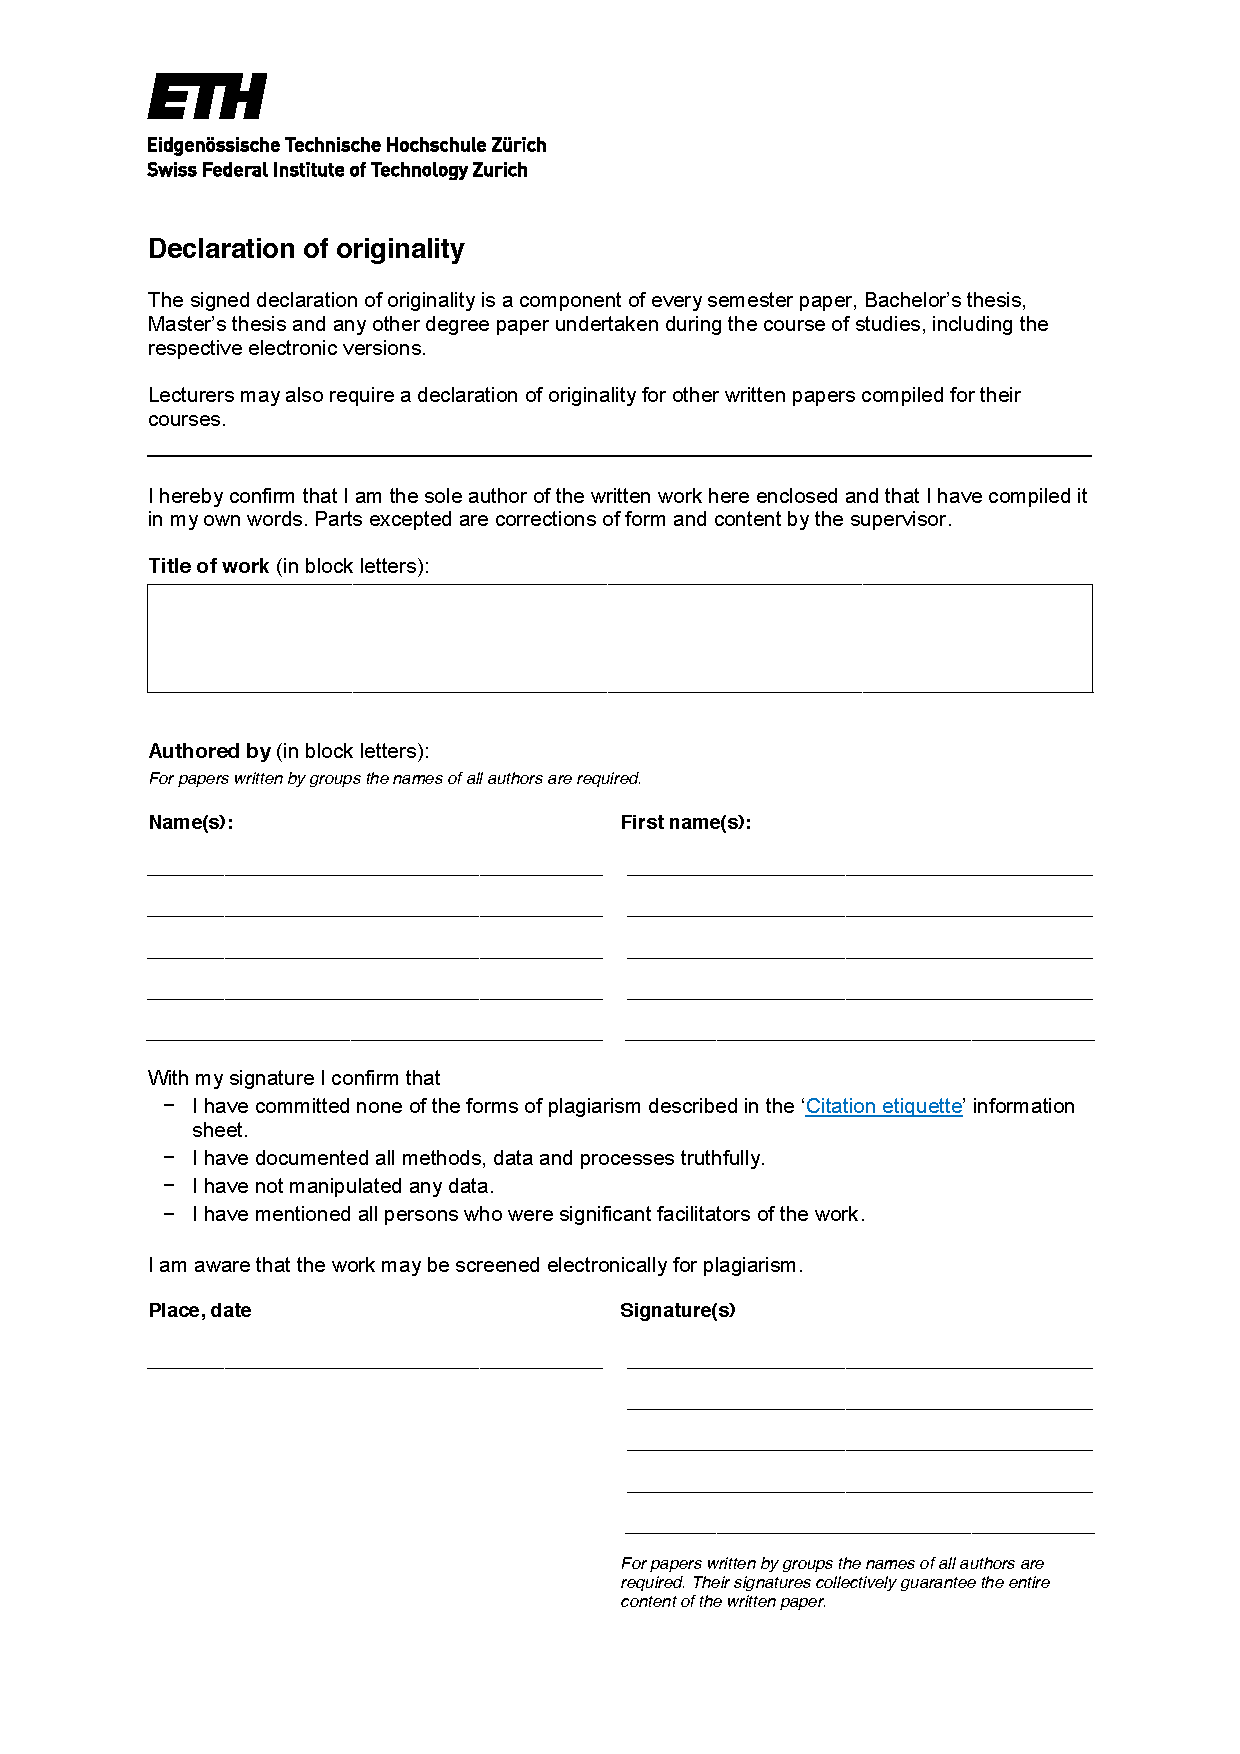
\includepdf[pages={-}]{declaration-originality.pdf}

\end{document}
